\documentclass[border=10pt]{standalone}
\usepackage{pgf,tikz,pgfplots}
\usetikzlibrary{quotes, angles}
%\usepackage{unicode-math}
%\setmainfont[Ligatures={TeX,Common}]{TeX Gyre Pagella}
%\setmathfont{TeX Gyre Pagella Math}
\usetikzlibrary{positioning}
\usetikzlibrary{arrows.meta}
\usetikzlibrary{calc, shapes, automata}
\tikzset{%
	% Specifications for style of nodes:
	base/.style = {rectangle, rounded corners, draw=black,
		inner sep=15pt,
		text centered, font=\sffamily}, 
	activityStarts/.style = {base, fill=blue!30},
	startstop/.style = {base, fill=red!30},
	activityRuns/.style = {base, fill=green!30},
	process/.style = {base, minimum width=2.5cm, fill=orange!15,
		font=\ttfamily},
}
\begin{document}
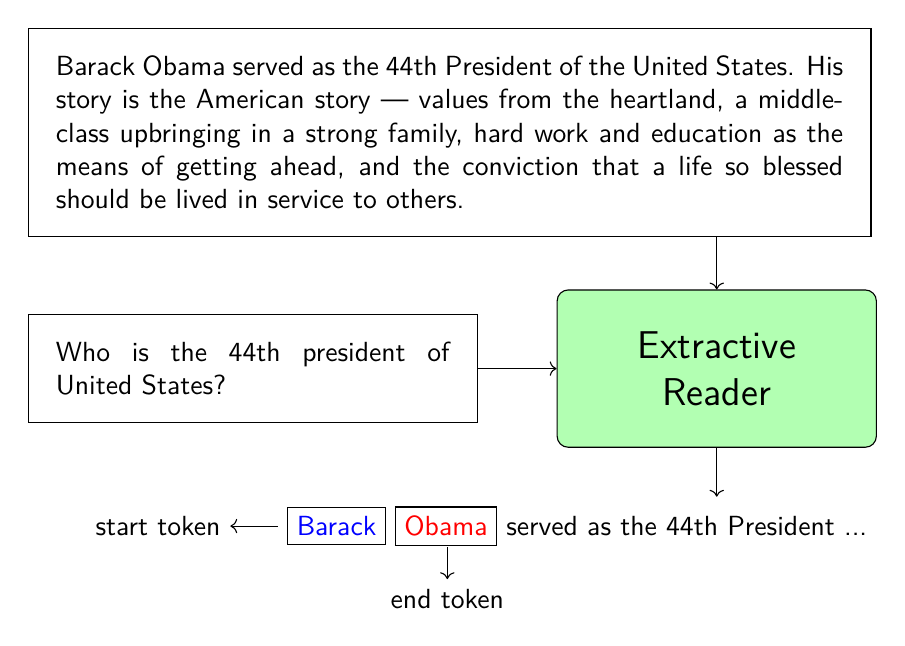
\begin{tikzpicture}[node distance=1.5cm,
	every node/.style={fill=white, font=\sffamily}, align=center]
	
\node (ctxs) [right, text width=10cm, align=justify, draw=black, inner sep=10pt] {Barack Obama served as the 44th President of the United States. His story is the American story — values from the heartland, a middle-class upbringing in a strong family, hard work and education as the means of getting ahead, and the conviction that a life so blessed should be lived in service to others.
};
\node (query) [right, draw=black, inner sep=10pt, align=justify, text width=5cm, below=3cm of ctxs.west, anchor=west] {Who is the 44th president of United States?};
\node (reader) [activityRuns, right=1.cm of query, text width=3.cm] {\fontsize{14pt}{\baselineskip}\selectfont Extractive\\[5pt] Reader};
\draw[->] (query) -- (reader);
\path let
	\p1 = (ctxs.south),
	\p2 = (reader.north)
in
	coordinate (ctxsAnchor) at (\x2, \y1);
\draw [->] (ctxsAnchor) -- (reader.north);
\node (output) [below=2.cm of reader.east, anchor=east] {\fbox{\textcolor{blue}{Barack}} \fbox{\textcolor{red}{Obama}} served as the 44th President ...};
\path let
	\p1 = (reader.south),
	\p2 = (output.north)
in
	coordinate (outputAnchor) at (\x1,\y2);
\draw[->] (reader.south) -- (outputAnchor);
\node (startToken) [left=.6cm of output.west] {start token};
\draw[->] (output.west) -- (startToken.east);
\node (endToken) [below=0.3cm of output.south, xshift=-1.65cm] {end token};
\path let
	\p1 = (output.south),
	\p2 = (endToken.north)
in 
	coordinate (endAnchor) at (\x2, \y1 + 3pt);
\draw[->] (endAnchor) -- (endToken.north);
\end{tikzpicture}
\end{document}